
% Somewhere: .map() for recoding

\chapter{\huge Associative arrays in Python (1 of 2)}
\label{ch:pythonAssocArrays}

\index{associative array}
\index{Pandas package}
\index{package}
\index{importing (a package)}

Our next trick is to represent associative arrays (review
section~\ref{sec:assocArrays} if you need to) in Python. To do so, we will
use another package, which goes by the adorable name ``Pandas'':

\begin{Verbatim}[fontsize=\small,samepage=true,frame=single,framesep=3mm]
import pandas as pd
\end{Verbatim}

This code should go at the top of your first notebook cell, right under your
``\texttt{import numpy as np}'' line. The two go hand in hand.

\index{table}
\index{NumPy package}
\index{series@\texttt{Series} (Pandas)}
\index{dict@\texttt{dict} (dictionary)}

By the way, just as there were other choices besides NumPy \texttt{ndarray}s to
represent ordinary arrays, there are other choices in Python for associative
arrays. The native Python \texttt{dict} (``dictionary'') is an obvious
candidate. Because this won't work well when the data gets huge, however, and
because using Pandas now will set up our usage of tables nicely in the next
few chapters, we're going to use the Pandas \textbf{Series} data type for our
associative arrays.


\section{The Pandas \texttt{Series}}
\label{sec:creatingSeries}

\index{array!associative}
\index{key-value pair}
\index{series@\texttt{Series} (Pandas)}

A \texttt{Series} is conceptually a set of key-value pairs. The keys are
normally homogeneous, and so are the values, although the keys might be of a
different type than the values. Any of the three atomic types are permissible
for either.

\index{index@index (pl:~indices)}
\index{deep}

Somewhat confusing is that the Pandas package calls the keys ``the
\textbf{index},'' which is an overlap with the term we used for ordinary arrays
(see p.~\ref{arrayIndex}). It's not a total loss, though, since if you think
hard about it, you'll realize that in some sense, \textit{a regular array is
really just an associative array with consecutive integer keys.} Oooo, deep. If
you consider the two halves of Figure~\ref{fig:assocArraysAreArrays}, I think
you'll agree.

\begin{figure}[ht]
\centering
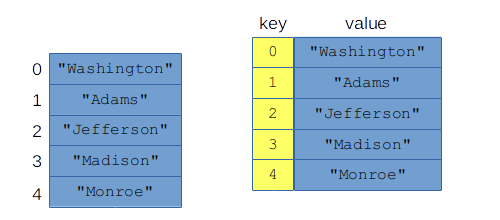
\includegraphics[width=0.9\textwidth]{assocArraysAreArrays.png}
\caption{An ordinary array, and an associative array, that represent the same
information.}
\label{fig:assocArraysAreArrays}
\end{figure}

\index{dimension}

\subsection{Creating \texttt{Series}es}

Here are a couple of common ways of creating a Pandas \texttt{Series} object in
memory.

\subsubsection{Way 1: \texttt{pd.Series([], index=[])}}

As with NumPy \texttt{ndarrays}, we can explicitly list the values we want in a
new \texttt{Series}. We also have to list the \textbf{index} values (the keys).
The syntax for doing so is:

\begin{Verbatim}[fontsize=\small,samepage=true,frame=single,framesep=3mm]
alter_egos = pd.Series(['Hulk','Spidey','Iron Man','Thor'],
    index=['Bruce','Peter','Tony','Thor'])
\end{Verbatim}

This creates the \texttt{Series} shown in Figure~\ref{fig:Series}.

\begin{figure}[ht]
\centering
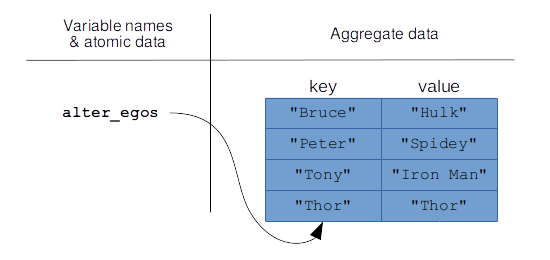
\includegraphics[width=0.8\textwidth]{Series.png}
\caption{A Pandas \texttt{Series} in memory.}
\label{fig:Series}
\end{figure}

\index{boxies (square brackets)}
\index{[]@\texttt{[]} (boxies)}
\index{bananas (parentheses)}
\index{()@\texttt{()} (bananas)}

Be careful to keep all your boxies and bananas straight. Note that both the
keys \textit{and} the values are in their own sets of boxies.

We can print (small) \texttt{Series}es to the screen to inspect their contents:

\begin{Verbatim}[fontsize=\small,samepage=true,frame=single,framesep=3mm]
print(alter_egos)
\end{Verbatim}

\begin{Verbatim}[fontsize=\small,samepage=true,frame=leftline,framesep=5mm,framerule=1mm]
Bruce        Hulk
Peter      Spidey
Tony     Iron Man
Thor         Thor
dtype: object
\end{Verbatim}

\index{type@\texttt{type()}}
\index{dtype@\texttt{.dtype} (NumPy/Pandas)}
and as we did on p.~\pageref{arrayType}, we can inquire as to both the
overarching type of \texttt{alter\_egos} and also to the kind of underlying
data it contains:

\begin{Verbatim}[fontsize=\small,samepage=true,frame=single,framesep=3mm]
print(type(alter_egos))
print(alter_egos.dtype)
\end{Verbatim}

\begin{Verbatim}[fontsize=\small,samepage=true,frame=leftline,framesep=5mm,framerule=1mm]
pandas.core.series.Series
object
\end{Verbatim}

Just as it did on p.~\pageref{dtypeRules}, the ``\texttt{object}'' here is just
a confusing way of saying ``\texttt{str}''. Don't read anything more into it
than that.

\subsubsection{Way 2: \texttt{pd.read\_csv()}}
